
% ============================================================
% Project : THE PHILOSOPHY OF VIABILITY
% Book    : Book I — Ontology of Viability
% Book ID : VS.B01
% Chapter : 08 — Comparative Philosophical Examination
% Section : 01 — Method and Criteria of Comparison
% Asset ID: VS.B01.P01.C08.S01.SS04.P009.DG01
% Type    : DG — Diagram
% File    : dialectical_comparison_cycle.tex
% Purpose : Represent the iterative and revisable structure
%           of the comparative dialectical procedure.
% ============================================================

\begin{figure}[htbp]
\centering

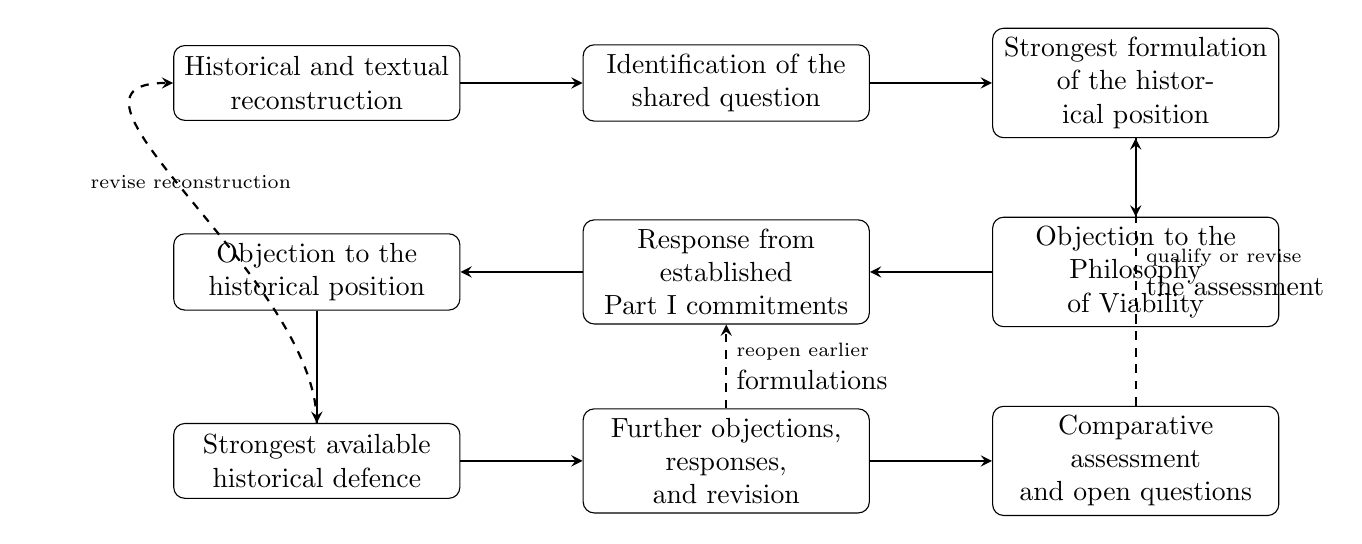
\begin{tikzpicture}[>=stealth]

% Nodes
\node[draw, rounded corners, align=center,
      text width=3.4cm, minimum height=0.95cm]
      (A) at (0,0)
      {Historical and textual\\reconstruction};

\node[draw, rounded corners, align=center,
      text width=3.4cm, minimum height=0.95cm]
      (B) at (5.2,0)
      {Identification of the\\shared question};

\node[draw, rounded corners, align=center,
      text width=3.4cm, minimum height=0.95cm]
      (C) at (10.4,0)
      {Strongest formulation\\of the historical position};

\node[draw, rounded corners, align=center,
      text width=3.4cm, minimum height=0.95cm]
      (D) at (10.4,-2.4)
      {Objection to the\\Philosophy of Viability};

\node[draw, rounded corners, align=center,
      text width=3.4cm, minimum height=0.95cm]
      (E) at (5.2,-2.4)
      {Response from established\\Part I commitments};

\node[draw, rounded corners, align=center,
      text width=3.4cm, minimum height=0.95cm]
      (F) at (0,-2.4)
      {Objection to the\\historical position};

\node[draw, rounded corners, align=center,
      text width=3.4cm, minimum height=0.95cm]
      (G) at (0,-4.8)
      {Strongest available\\historical defence};

\node[draw, rounded corners, align=center,
      text width=3.4cm, minimum height=0.95cm]
      (H) at (5.2,-4.8)
      {Further objections,\\responses, and revision};

\node[draw, rounded corners, align=center,
      text width=3.4cm, minimum height=0.95cm]
      (I) at (10.4,-4.8)
      {Comparative assessment\\and open questions};

% Main argumentative movement
\draw[->, thick] (A) -- (B);
\draw[->, thick] (B) -- (C);
\draw[->, thick] (C) -- (D);
\draw[->, thick] (D) -- (E);
\draw[->, thick] (E) -- (F);
\draw[->, thick] (F) -- (G);
\draw[->, thick] (G) -- (H);
\draw[->, thick] (H) -- (I);

% Revision and feedback relations
\draw[->, dashed, thick]
  (G.north) to[out=90,in=180]
  node[above, align=center]
  {\scriptsize revise reconstruction}
  (A.west);

\draw[->, dashed, thick]
  (H.north) to[out=90,in=270]
  node[right, align=left]
  {\scriptsize reopen earlier\\formulations}
  (E.south);

\draw[->, dashed, thick]
  (I.north) to[out=90,in=270]
  node[right, align=left]
  {\scriptsize qualify or revise\\the assessment}
  (C.south);

\end{tikzpicture}

\caption{The iterative dialectical procedure of comparative examination. The arrows represent the principal argumentative sequence and the dashed arrows represent possible revision and feedback. The diagram does not imply that every comparison must terminate in a final resolution.}
\label{fig:ch08-dialectical-comparison-cycle}

\end{figure}

% ============================================================
% END OF ASSET
% ============================================================
